\section{Результаты}
Параметры окружающей среды при проведении эксперимента
\[T = 296K\]
\[P = 101295\text{Па}\]

В работе использована экспериментальная установка, состоящая из компрессора, газового счетчика и нескольких тонких металлических трубок. Воздух нагнетался компрессором и пропускался через трубки. Интенсивность потока регулировалась краном. Трубки оснащены рядом миллиметровых отверстий, к которым можно подключать микроманометр. (Измерения проводились при условиях ...)Более подробное описание экспериментальной установки см. в \nameref{Приложение 1}.

Для определения разности давления на выделенном участке трубки использовался спиртовой микроманометр ММН-2400 с регулируемым наклоном, который подключался к отверстиям в трубке. Подробное описание устройства микроманометра см. в \nameref{Приложение 2}.

Для измерения расхода газа использовался газовый счетчик ГСБ-400. Подробное описание устройства газового счетчика см. в \nameref{Приложение 3}.

Перед проведением измерений был измерен критический расход $Q_\text{кр}$ воздуха, при котором число Рейнольдса $Re \approx 10^3$, для нескольких трубок.
Результаты представлены ниже
\[Q_\text{кр} = 6.4\frac{\text{л}}{\text{мин}} \](для трубки диаметром $d = 3.95\text{мм}$)
\[Q_\text{кр} = 8.18\frac{\text{л}}{\text{мин}} \](для трубки диаметром $d = 5.05\text{мм}$)

Способ вычисления представлен в \nameref{Приложение 5}.

Также с помощью выражения \eqref{eq: l_ust} была вычислена длина установления Пуазейлевского течения для трубок различного диаметра
Для трубки диаметром ... длина составила ...
\[ l_\text{уст} = 39.5\text{см}\] (трубка диаметром $d = 3.95\text{мм}$)
\[ l_\text{уст} = 50.5\text{см}\] (трубка диаметром $d = 5.05\text{мм}$)

По измеренным зависимостям расхода $Q$ воздуха от перепада давления $\Delta P$ на выделенном участке трубки длиной $l$ для двух трубок разного диаметра (см. таблицы 2 и 3 \nameref{Приложение 4}) построены графики $Q(\Delta P)$ (см. рис. 1, 2).
\newpage
\begin{figure}[ht]
    \label{figure5}
    \center{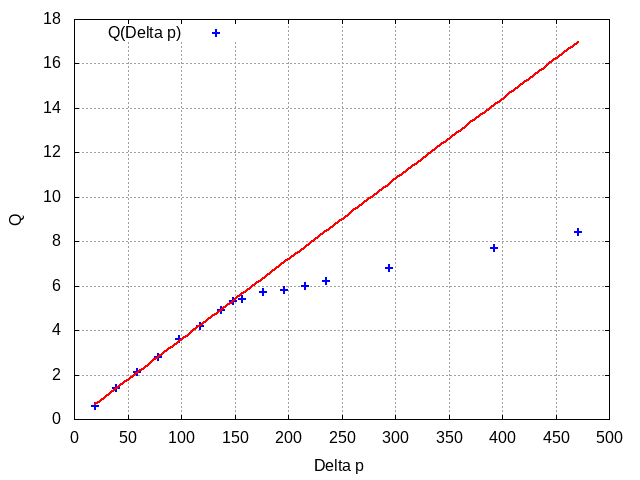
\includegraphics[scale=0.7]{img/graph13.png}}
    \caption{График зависимости расхода $Q$ воздуха от перепада давления $\Delta P$ в трубке диаметром $d = 3.95\text{мм}$}
\end{figure}
\begin{figure}[ht]
    \label{figure6}
    \center{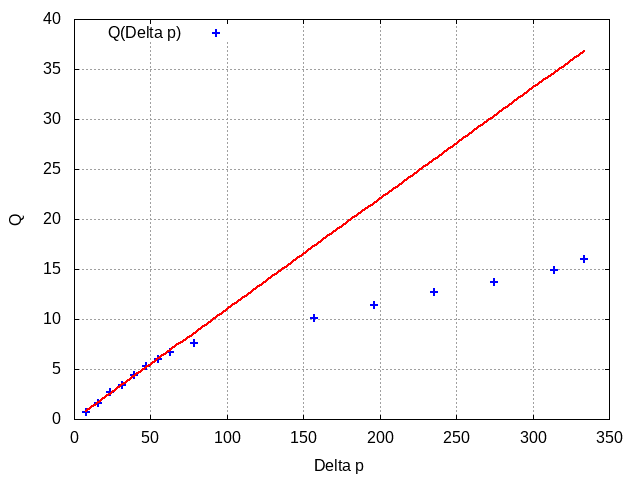
\includegraphics[scale=0.7]{img/graph14.png}}
    \caption{График зависимости расхода $Q$ воздуха от перепада давления $\Delta P$ в трубке диаметром $d = 5.05\text{мм}$}
\end{figure}
\newpage
На обоих графиках присутствует начальный участок с линейной зависимостью расхода от перепада давления. На этом участке выполняется формула Пуазейля \eqref{eq: Q} и течение является ламинарным. Область графика, в которой пропадает линейная зависимость, обозначает, что характер течения сменился на турбулентный.

По угловому коэффициенту линейных участков графиков и выражению \eqref{eq: Q} определили коэффициент вязкости воздуха $\eta$.

\begin{table}[ht]
\centering
\begin{tabular}{|c|c|c|}
 \hline
$d, \text{мм}$ & $\eta, \cdot 10^{-5} \text{Па}\cdot \text{c}$ & Re \\
 \hline
3.95 & $2.0 \pm 0.2$ & $1560 \pm 160$\\ \hline
5.05 & $1.7 \pm 0.4$ & $1600 \pm 400$\\ \hline
\end{tabular}
\caption{Коэффициенты вязкости $\eta$ воздуха, полученные для каждой трубки диаметром $d$ из формулы Пуазейля с использованием коэффициента наклона линейной части графиков зависимости расхода воздуха Q от разности давлений $\Delta P$. $Re$ - число Рейнольдса.}
\end{table}

С учетом погрешности коэффициент вязкости не зависит от диаметра трубки и равен $\eta = (1.85 \pm 0.3)\text{Па}\cdot\text{с}$. Значение $\eta$ в пределах погрешности совпало с табличным (\nameref{Приложение 7}).

Измерили распределение давления воздуха в трубке. Для этого установили расход воздуха, близкий к критическому, но всё еще сохраняющий ламинарность. Не меняя расхода, подсоединяли микроманометр ко всем парам отверстий исследуемой трубки и измеряли соответствующие перепады давлений. Результаты измерений приведены в таблицах 5, 6. По измеренным зависимостям построены графики (рис. 3, 4).

\begin{figure}[ht]
    \label{figure7}
    \center{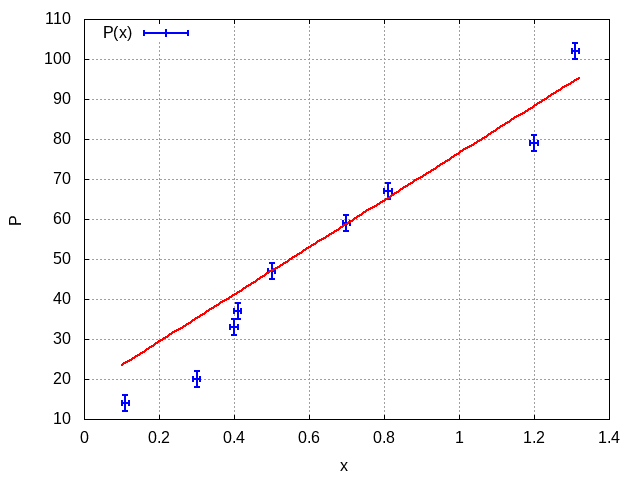
\includegraphics[scale=0.7]{img/graph15.png}}
    \caption{График зависимости давления $P$ воздуха трубке от расстояния $x$ до входа в трубку, диаметр трубки $d = 3.95\text{мм}$}
\end{figure}
\begin{figure}[ht]
    \label{figure8}
    \center{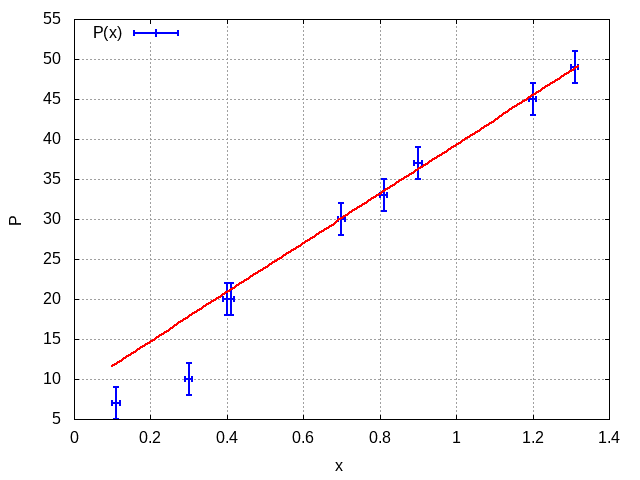
\includegraphics[scale=0.7]{img/graph16.png}}
    \caption{График зависимости давления $P$ воздуха трубке от расстояния $x$ до входа в трубку, диаметр трубки $d = 5.05\text{мм}$}
\end{figure}
\newpage

Линейные участки графиков обозначают, что на данном расстоянии от входа в трубку течение воздуха является установившимся. По графикам определили $l_\text{уст}$ для двух трубок.
\begin{table}[ht]
\begin{tabular}{|c|c|c|}
 \hline
$d, \text{мм}$ & $l_\text{уст}, \text{см}$ & $l_\text{уст}$ по формуле, \text{см} \\ \hline
3.95 & 40 & 39.5  \\  \hline
5.05 & 50 & 50.5  \\ \hline
\end{tabular}
\caption{Значение длины установления потока в трубках различного диаметра}
\end{table}

Полученные значения разошлись со значениями, вычисленными через \eqref{eq: l_ust}, менее чем на 2\%. Значит, метод оценки \eqref{eq: l_ust} позволяет вычислить длину установления с точностью до 2\%. (Таким образом, использованный метод позволяет получить точность ... процентов)

Для проверки выполнимости выражений \eqref{eq: Q} и \eqref{eq: Q1} для ламинарного и турбулентного течений, полученных из теории, определили коэффициент $\beta$, связывающий расход и радиус трубки:$Q \propto r^\beta$. Результаты измерения зависимости расхода $Q$ воздуха от диаметра $d$ трубки при постоянном градиенте давления $\frac{\Delta P}{l}$ представлены в таблице 3.

\begin{table}[ht]
\centering
\label{tab:flow_regimes}
\begin{tabular}{|c|c|c|c|c|c|}
\hline
\multicolumn{3}{|c|}{\textbf{Ламинарный режим}} & \multicolumn{3}{c|}{\textbf{Турбулентный режим}} \\ \hline
$d$, мм & $\Delta P/l$, Па/см & $Q$, л/мин & $d$, мм & $\Delta P/l$, Па/см & $Q$, л/мин \\ \hline
3.95 & $0.980 \pm 0.019$ & $7.80 \pm 0.08$ & 3.95 & $5.88 \pm 0.05$ & $6.80 \pm 0.07$ \\ \hline
5.05 & $0.980 \pm 0.019$ & $11.80 \pm 0.12$ & 5.05 & $5.88 \pm 0.05$ & $14.20 \pm 0.14$ \\ \hline
\end{tabular}
\caption{Зависимость рсхода $Q$ воздуха от диаметра $d$ трубки при постоянном градиенте давления $\frac{\Delta P}{l}$}
\end{table}
\newpage
По таблице 3 определили, что $\beta_{\text{л}} = 1.7$ для ламинарного течения, $\beta_{\text{т}} = 3.0$ для турбулентного течения. Это означает, что теоретическая модель (ссылка) описания турбулентного течения, основанная на том, что флуктуации скорости по порядку величины совпадают со средней скоростью потока и элементы жидкости равномерно перемешиваются по сечению трубы, и метод размерностей для ламинарного течения не применимы для данного эксперимента.